\documentclass{article}

\usepackage{graphicx} % Required for inserting images
\usepackage[left=1in,right=1in,top=1in,bottom=1in]{geometry} \usepackage{amsmath}
\usepackage{amsthm} %proof environment
\usepackage{amsthm} %proof environment
\usepackage{amssymb}
\usepackage{amsfonts}
\usepackage{enumitem} %nice lists
\usepackage{verbatim} %useful for something 
\usepackage{xcolor}
\usepackage{setspace}
\usepackage{titlesec}
\usepackage{blindtext} % I have no idea what this is 
\usepackage{caption}  % need this for unnumbered captions/figures
\usepackage{natbib}
\usepackage{appendix}
\usepackage{tikz}
\usepackage{hyperref}


\hypersetup{
    colorlinks=true,
    linkcolor=blue,
    filecolor=magenta,      
    urlcolor=blue,
    pdftitle={Overleaf Example},
    pdfpagemode=FullScreen,
    }

\titleformat{\section}{\bfseries\Large}{Problem \thesection:}{5pt}{}

\begin{document}

\title{AM 260 - Computational Fluid Dynamics: Homework 3}
\author{Dante Buhl}


\newcommand{\wrms}{w_{\text{rms}}}
\newcommand{\bs}[1]{\boldsymbol{#1}}
\newcommand{\tb}[1]{\textbf{#1}}
\newcommand{\bmp}[1]{\begin{minipage}{#1\textwidth}}
\newcommand{\emp}{\end{minipage}}
\newcommand{\R}{\mathbb{R}}
\newcommand{\C}{\mathbb{C}}
\newcommand{\N}{\mathcal{N}}
%\newcommand{\K}{\bs{\mathrm{K}}}
\newcommand{\m}{\bs{\mu}_*}
\newcommand{\s}{\bs{\Sigma}_*}
\newcommand{\dt}{\Delta t}
\newcommand{\dx}{\Delta x}
\newcommand{\tr}[1]{\text{Tr}(#1)}
\newcommand{\Tr}[1]{\text{Tr}(#1)}
\newcommand{\Div}{\nabla \cdot}
\renewcommand{\div}{\nabla \cdot}
\newcommand{\Curl}{\nabla \times}
\newcommand{\Grad}{\nabla}
\newcommand{\grad}{\nabla}
\newcommand{\grads}{\nabla_s}
\newcommand{\gradf}{\nabla_f}
\newcommand{\xs}{x_s}
\newcommand{\x}{\bs{x}}
\newcommand{\xf}{x_f}
\newcommand{\ts}{t_s}
\newcommand{\tf}{t_f}
\newcommand{\pt}{\partial t}
\newcommand{\pz}{\partial z}
\newcommand{\uvec}{\bs{u}}
\newcommand{\bvec}{\bs{B}}
\newcommand{\nvec}{\hat{\bs{n}}}
\newcommand{\tu}{\tilde{\uvec}}
\newcommand{\B}{\bs{B}}
\newcommand{\A}{\bs{A}}
\newcommand{\jvec}{\bs{j}}
\newcommand{\F}{\bs{F}}
\newcommand{\T}{\tilde{T}}
\newcommand{\ez}{\bs{e}_z}
\newcommand{\ex}{\bs{e}_x}
\newcommand{\ey}{\bs{e}_y}
\newcommand{\eo}{\bs{e}_{\bs{\Omega}}}
\newcommand{\ppt}[1]{\frac{\partial #1}{\partial t}}
\newcommand{\pp}[2]{\frac{\partial #1}{\partial #2}}
\newcommand{\pptwo}[2]{\frac{\partial^2 #1}{\partial #2^2}}
\newcommand{\ddtwo}[2]{\frac{d^2 #1}{d #2^2}}
\newcommand{\DDt}[1]{\frac{D #1}{D t}}
\newcommand{\ppts}[1]{\frac{\partial #1}{\partial t_s}}
\newcommand{\pptf}[1]{\frac{\partial #1}{\partial t_f}}
\newcommand{\ppz}[1]{\frac{\partial #1}{\partial z}}
\newcommand{\ddz}[1]{\frac{d #1}{d z}}
\newcommand{\ppzetas}[1]{\frac{\partial^2 #1}{\partial \zeta^2}}
\newcommand{\ppzs}[1]{\frac{\partial #1}{\partial z_s}}
\newcommand{\ppzf}[1]{\frac{\partial #1}{\partial z_f}}
\newcommand{\ppx}[1]{\frac{\partial #1}{\partial x}}
\newcommand{\ddx}[1]{\frac{d #1}{d x}}
\newcommand{\ppxi}[1]{\frac{\partial #1}{\partial x_i}}
\newcommand{\ppxj}[1]{\frac{\partial #1}{\partial x_j}}
\newcommand{\ppy}[1]{\frac{\partial #1}{\partial y}}
\newcommand{\ppzeta}[1]{\frac{\partial #1}{\partial \zeta}}
\renewcommand{\k}{\bs{k}}
\newcommand{\real}[1]{\text{Re}\left[#1\right]}


\maketitle 
% This line removes the automatic indentation on new paragraphs
\setlength{\parindent}{0pt}

\section{Lax-Friedrichs Method}

\begin{enumerate}[label = (\alph*)]
    \item Show that the LW method is convergent if $|C_a| \le 1$. 

    \textbf{Consistency}
        Here are the taylor expansions which will be used to show consistency
        both for 1.a. and 2.a.
        \begin{align*}
            U_j^{n+1} &= U_j^n + \Delta t U_{t, j}^n + 
            \frac{\Delta t^2}{2}U_{tt, j}^n + \frac{\Delta t^3}{6}U_{ttt, j}^n
            + \frac{\Delta t^4}{24}U_{tttt, j}^n + O(\Delta t^5)\\
            U_{j+1}^{n} &= U_j^n + \Delta x U_{x, j}^n + 
            \frac{\Delta x^2}{2}U_{xx, j}^n + \frac{\Delta x^3}{6}U_{xxx, j}^n
            + \frac{\Delta x^4}{24}U_{xxxx, j}^n + O(\Delta x^5)\\
            U_{j-1}^{n} &= U_j^n - \Delta x U_{x, j}^n + 
            \frac{\Delta x^2}{2}U_{xx, j}^n - \frac{\Delta x^3}{6}U_{xxx, j}^n
            + \frac{\Delta x^4}{24}U_{xxxx, j}^n + O(\Delta x^5)
        \end{align*}
        \begin{align*}
            \Delta t E_{LT} &= 
            U_j^n + \Delta t U_{j, t}^n + \frac{\Delta t^2}{2} U_{j, tt}^n +
            \ldots \\
            &-\frac{1}{2}\left(U_j^n + \Delta x U_{j, x}^n + \frac{\Delta
            x^2}{2}U_{j, xx}^n + \ldots\right)\\
            &-\frac{1}{2}\left(U_j^n - \Delta x U_{j, x}^n + \frac{\Delta
            x^2}{2}U_{j, xx}^n + \ldots\right) \\
            &+\frac{a\Delta t}{2\Delta x}\left(U_j^n + \Delta x U_{j, x}^n + \frac{\Delta
            x^2}{2}U_{j, xx}^n + \ldots\right)\\
            &-\frac{a\Delta t}{2\Delta x}\left(U_j^n - \Delta x U_{j, x}^n + \frac{\Delta
            x^2}{2}U_{j, xx}^n + \ldots\right)\\
        \end{align*}
        \begin{gather*}
            \lim_{\Delta t, \Delta x \to 0} E_{LT} = \lim_{\Delta t, \Delta x
            \to 0} \frac{1}{\Delta t}\left( U_j^{n+1} - 
            \frac{1}{2}\left(U_{j+1}^n + U_{j-1}^n\right) + \frac{a\Delta
            t}{2\Delta x}\left(U_{j+1}^n - U_{j-1}^n\right)\right)\\
            = \lim_{\Delta t, \Delta x \to 0} U_{t, j}^n + 
            \frac{\Delta t}{2}U_{tt, j}^n + O(\Delta t^2) 
            + \frac{\Delta x^2}{2\Delta t}U_{xx, j}^n + O(\Delta x^3) +
            U_{x, j}^n + \frac{\Delta x^2}{6}U_{xxx,j}^n\\
            = \lim_{\Delta t, \Delta x \to 0}\frac{\Delta t}{2}U_{tt, j}^n+ 
            \frac{\Delta x}{2a}U_{xx, j}^n + O(\Delta^2)
        \end{gather*}
        Therefore, we have shown that the local truncation error is bounded by
        $\Delta t + \Delta x$ with order 1. 

    \textbf{Stability}
    Next to show stability we look at the von Neumann stability analysis. We
    have, 
    \begin{gather*}
        G = \frac{1}{2}\left(e^{ik_x\Delta x} + e^{-ik+x\Delta x}\right) -
        \frac{C_a}{2}\left(e^{ik_x\Delta x} - e^{-ik+x\Delta x}\right)\\
        = \cos(k_x\Delta x) - iC_a\sin(k_x\Delta x)\\
        |G| = \cos^2(k_x\Delta x) + C_a^2\sin^2(k_x\Delta x)\\
        = \cos^2(k_x\Delta x) + \sin^2(k_x\Delta x) + (C_a^2 -1)\sin^2(k_x\Delta
        x) = 1 - (1 - C_a^2)\sin^2(k_x\Delta
        x) \le 1
    \end{gather*}
    Where here, since $|C_a| \le 1$  we must have that $C_a^2 \le 1$ and the
    right most term is negative semi-definite, thereby bounding $|G|$ to ensure
    stability. 

    \item Show that the LF method is $O(\Delta t + \Delta x)$. 

    This has been shown in the proof for consistency in 1.a.

    \item Rewrite the LF method in the conservative form, 

    In order to solve for the fluxes $\hat{f}_{i+1/2}^n$ we will first solve for
    $\hat{f}_{i+1/2}^n - \hat{f}_{i-1/2}^n$ and then isolate each term using
    addition. 
    \begin{gather*}
        \hat{f}_{i+1/2}^n - \hat{f}_{i-1/2}^n = -\frac{\Delta x}{\Delta
        t}\left(\frac{1}{2}U_{i+1}^n - U_{i}^n + \frac{1}{2}U_{i-1}^n\right) +
        \frac{1}{2}\left(f(U_{i+1}^n - f(U_{i-1}^n)\right)
    \end{gather*}
    Since this holds for any arbitrary $i$ we can add additional terms to this
    sum in order to increase the distance between the terms on the LHS. 
    \begin{align*}
        \hat{f}_{i+1/2}^n - \hat{f}_{i-1/2}^n &= -\frac{\Delta x}{\Delta
        t}\left(\frac{1}{2}U_{i+1}^n - U_{i}^n + \frac{1}{2}U_{i-1}^n\right) +
        \frac{1}{2}\left(f(U_{i+1}^n) - f(U_{i-1}^n)\right)\\
        \hat{f}_{i+3/2}^n - \hat{f}_{i+1/2}^n &= -\frac{\Delta x}{\Delta
        t}\left(\frac{1}{2}U_{i+2}^n - U_{i+1}^n + \frac{1}{2}U_{i}^n\right) +
        \frac{1}{2}\left(f(U_{i+2}^n) - f(U_{i}^n)\right)\\
        \hat{f}_{i-1/2}^n - \hat{f}_{i-3/2}^n &= -\frac{\Delta x}{\Delta
        t}\left(\frac{1}{2}U_{i}^n - U_{i-1}^n + \frac{1}{2}U_{i-2}^n\right) +
        \frac{1}{2}\left(f(U_{i}^n) - f(U_{i-2}^n)\right)
    \end{align*}
    Adding these three equations together, we find some terms cancel. We have
    remaining, 
    \begin{gather*}
        \hat{f}_{i+3/2}^n - \hat{f}_{i-3/2}^n = -\frac{\Delta x}{2\Delta
        t}\left(U_{i+2}^n - U_{i+1}^n +
        U_{i-2}^n - U_{i-1}^n\right) +
        \frac{1}{2}\left(f(U_{i+2}^n) + f(U_{i+1}^n) - f(U_{i-2}^n) - f(U_{i-1}^n)\right)
    \end{gather*}
    We are able to deduce the value for each of the LHS terms separately using
    symmetry and by the fact that each flux should only have information from
    the two indices adjacent ($i + 3/2$ should only be influenced by $i + 1,
    i+2$ and similar argument for $i-3/2$). Thus we have,
    \begin{align*}
        \hat{f}_{i+3/2}^n &= -\frac{\Delta x}{2\Delta
        t}\left(U_{i+2}^n - U_{i+1}^n\right) + 
        \frac{1}{2}\left(f(U_{i+2}^n) + f(U_{i+1}^n)\right)\\
        \hat{f}_{i+1/2}^n &= -\frac{\Delta x}{2\Delta
        t}\left(U_{i+1}^n - U_{i}^n\right) + 
        \frac{1}{2}\left(f(U_{i+1}^n) + f(U_{i}^n)\right)
    \end{align*}



\end{enumerate}

\section{Lax-Wendroff Method}

\begin{enumerate}[label = (\alph*)]
    \item Show that the LW method is convergent if $|C_a| \le 1$. 
    
        In order to demonstrate consistency and stability, we perform taylor
        expansions to demonstrate consistency (and at which order it is
        consistent), and then von Neumann stability analysis in order to prove
        stability.

        \textbf{Consistency}
        \begin{gather*}
            \lim_{\Delta t, \Delta x \to 0} E_{LT} = 
            \lim_{\Delta t, \Delta x \to 0} \frac{1}{\Delta t} U_j^{n+1} - U_j^n
            + \frac{1}{2}C_a\left(U_{j+1}^n - U_{j-1}^n\right)
            - \frac{1}{2}C_a^2\left(U_{j+1}^n - 2U_j^n + U_{j-1}^n\right)\\
           =  \lim_{\Delta t, \Delta x \to 0} U_{t, j}^n + 
            \frac{\Delta t}{2}U_{tt, j}^n + \frac{\Delta t^2}{6}U_{ttt, j}^n +
            O(\Delta t^3)
            + aU_{x, j}^n + a\frac{\Delta
            x^2}{6}U_{xxx, j}^n + O(\Delta x^4) \\- aC_a\left(
            \frac{\Delta x}{2}U_{xx, j}^n + \frac{\Delta x^3}{24}U_{xxxx, j}^n
            + O(\Delta x^5)\right)\\
            = \lim_{\Delta t, \Delta x \to 0} \frac{\Delta t^2}{6}U_{ttt, j}^n +
            a \frac{\Delta x^2}{6}U_{xxx, j}^n + O(\Delta^3)
        \end{gather*}
        Therefore, we have that this method is consistent with $O(\Delta t^2 +
        \Delta x^2)$. 

        \textbf{Stability} 
        \begin{gather*}
            G = (1 - C_a^2) + \frac{1}{2}\left(C_a^2 - C_a\right) e^{ik_x\Delta
            x} + \frac{1}{2}\left(C_a^2 + C_a\right) e^{-ik_x\Delta x}\\
            G = (1 - C_a^2) + C_a^2\cos(k_x \Delta x) - iC_a\sin(k_x \Delta x)\\
            |G| = (1 - C_a^2)^2 + C_a^4\cos^2(k_x \Delta x) + 2(1 -
            C_a^2)C_a^2\cos(k_x\Delta x) + C_a^2\sin^2(k_x\Delta x)\\
            = 1 - 2C_a^2 + C_a^4 + C_a^4\cos^2() + 2C_a^2\cos() - 2C_a^4\cos() +
            C_a^2\sin^2()\\
            = 1 + C_a^2\left(2\cos + \sin^2 - 2\right) + C_a^4\left(1 + \cos^2 -
            2\cos\right)
        \end{gather*}
        We proceed from here casewise. Take, $|C_a| = 1$. We have, 
        \begin{gather*}
            |G| = 1 + 2\cos - 2 + 1 - 2\cos + 1 = 1
        \end{gather*}
        in which case, the method is stable. 
        We next consider $|C_a| \le 1$, for this case, it is hard to simplify
        the RHS (due to the Sinusoidal terms)
        in order to show that $|G| - 1$ is negative semi-definite. This
        can however easily be verified using any plotting routine. 
        \href{https://www.desmos.com/calculator/znn8cfqqxg}{Here is a
        link} to a desmos graph which shows an animation of $|G| - 1$ and
        demonstrates the fact that it is a negative semi-definite term . 

    

    \item Show that the LW method is $O(\Delta t^2 + \Delta x^2)$.

    This has already been shown in the proof for consistency of the Lax-Wendroff
    method, whereby the Local Truncation Error is shown to be bounded by $\Delta
    t^2$ and $\Delta x^2$. 
\end{enumerate}

\section{von Neumann Stability Analysis}
We can show that this method is unconditionally unstable with only a few lines
of algebra. 
\begin{gather*}
    U_j^{n+1} = U_j^n - \frac{a\Delta t}{2\Delta x}\left(U_{j+1}^n -
    U_{j-1}^n\right), \quad U_{j}^n = G^ne^{i j k_x \Delta x}\\
    G = 1 - \frac{a\Delta t}{2\Delta x}\left(e^{ik_x\Delta x}  - e^{-ik_x\Delta
    x}\right)\\
    G = 1 - \frac{a\Delta t}{2\Delta x}i\sin(k_x\Delta x)\\
    |G| = 1 + \left(\frac{a\Delta t}{2\Delta x}\right)^2\sin(k_x\Delta x)^2 > 1
\end{gather*}
Therefore, we have that this method is unconditionally unstable, i.e. there is
no condition on which $|G| \le 1$. 

\section{Modified Lax-Friedrichs Coefficient}

We show the diffusion coefficient for the Lax-Friedrichs method by taylor
expanding the original PDE. 
\begin{gather*}
    \Delta t u_t(x,t) + \frac{\Delta t^2}{2} u_{tt}(x,t)  =
    \frac{1}{2}\left(\Delta x^2u_{xx}(x,t) + \frac{\Delta x^4}{12} \right) -
    \frac{C_a}{2}\left(2\Delta x u_x + \frac{\Delta x^3}{3}u_{xxx}(x,t) \right)\\
    u_t + a u_x = - \frac{\Delta t}{2} u_{tt} + \frac{\Delta x^2}{2\Delta
    t}u_{xx} - \frac{a\Delta x^2}{6\Delta t}u_{xxx} + O(\Delta x^4, \Delta
    t^2)\\
    u_t + a u_x = \frac{\Delta x^2}{2\Delta t}\left(-\frac{a^2\Delta t^2}{\Delta
    x^2} + 1\right)u_{xx} + O(\Delta x^2, \Delta t^2)\\
    \kappa = \frac{\Delta x^2}{2\Delta t}\left(1-\frac{a^2\Delta t^2}{\Delta
    x^2}\right)
\end{gather*}

This diffusion coefficient is interesting because it is inversely proportional
to the temporal discretization, i.e. smaller timesteps make the method more
diffuse. This will cause the velocity field to dampen more quickly as the
timestep becomes smaller. At the same time it is stabilized by the gridsize,
i.e. smaller spatial discretizations will cause the diffusion coefficient to
become smaller (as it varies proportional to the square of $\Delta x$). 

\section{von Neumann Analysis of the Heat Equation}

In order to show this, we substitute the von Neumann ansatz into the update
function.  
\begin{gather*}
    G = 1 + C_k\left(e^{ik_x\Delta x} - 2 + e^{-ik_x\Delta x}\right)\\
    G = 1 - 2C_k + 2C_k\cos(k_x\Delta x) \\
    G = 1 + 2C_k(\cos(k_x\Delta x) -1))\\
    1 - 4C_k \le G \le 1,\quad |G| \le 1  \implies C_k \le 0.5
\end{gather*}

\begin{figure}[t]
    \centering
    \bmp{.49}
        \centering
        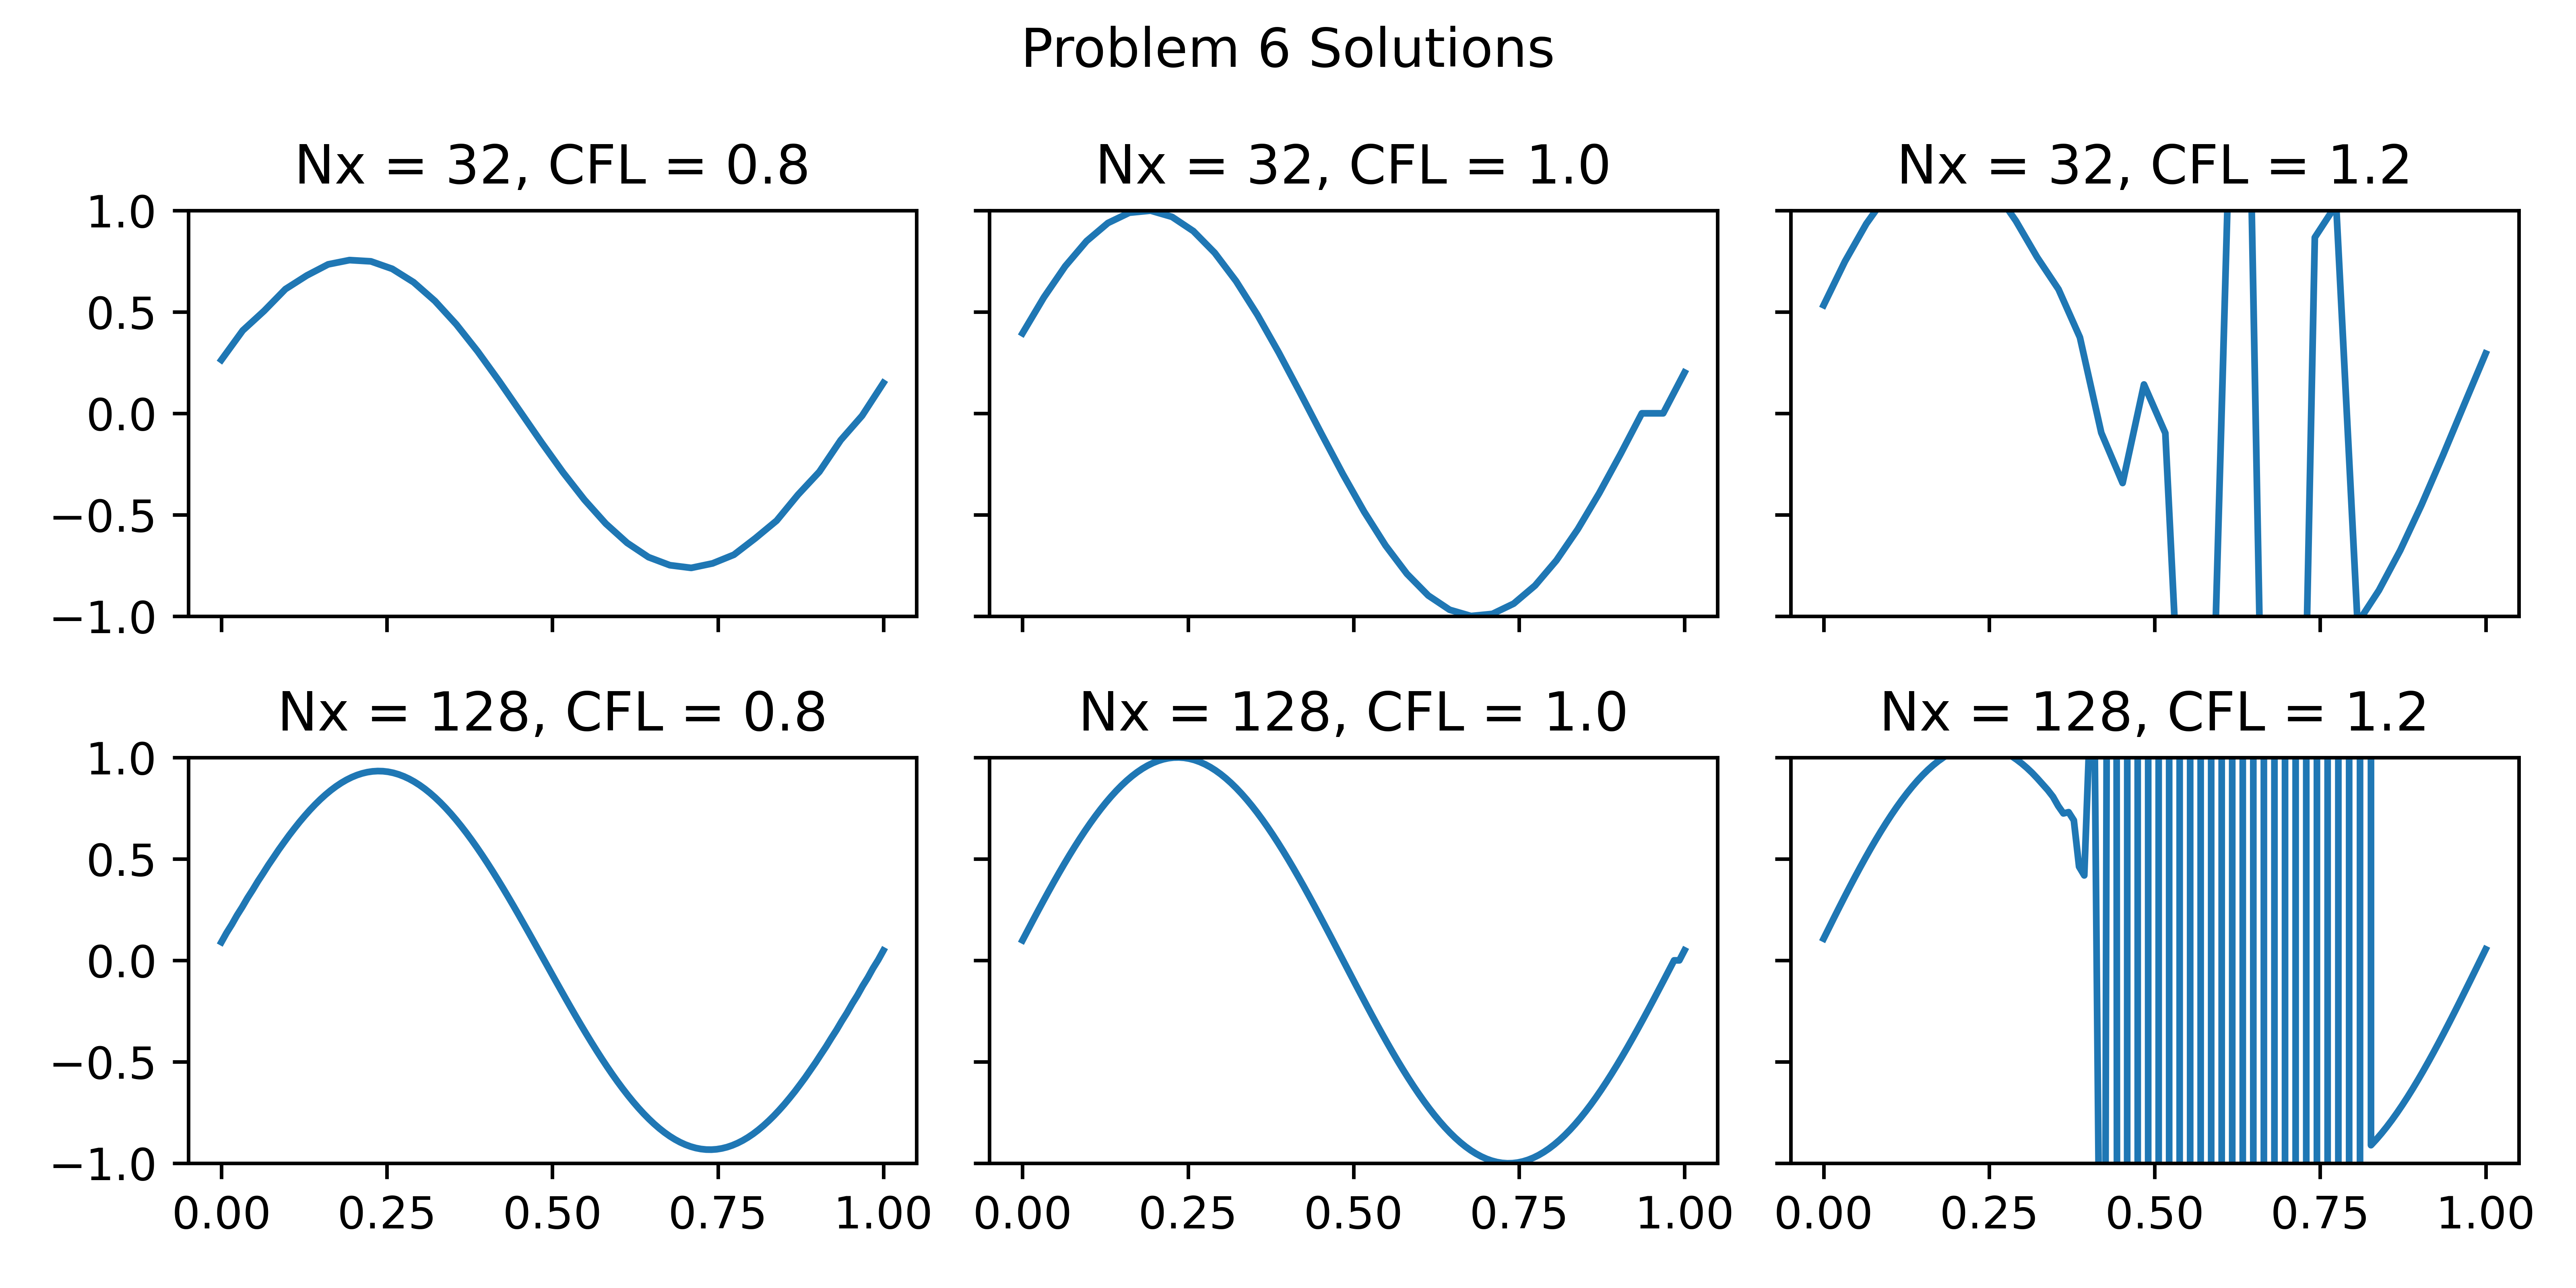
\includegraphics[width=\textwidth]{../code/prob6_tstop.png}
        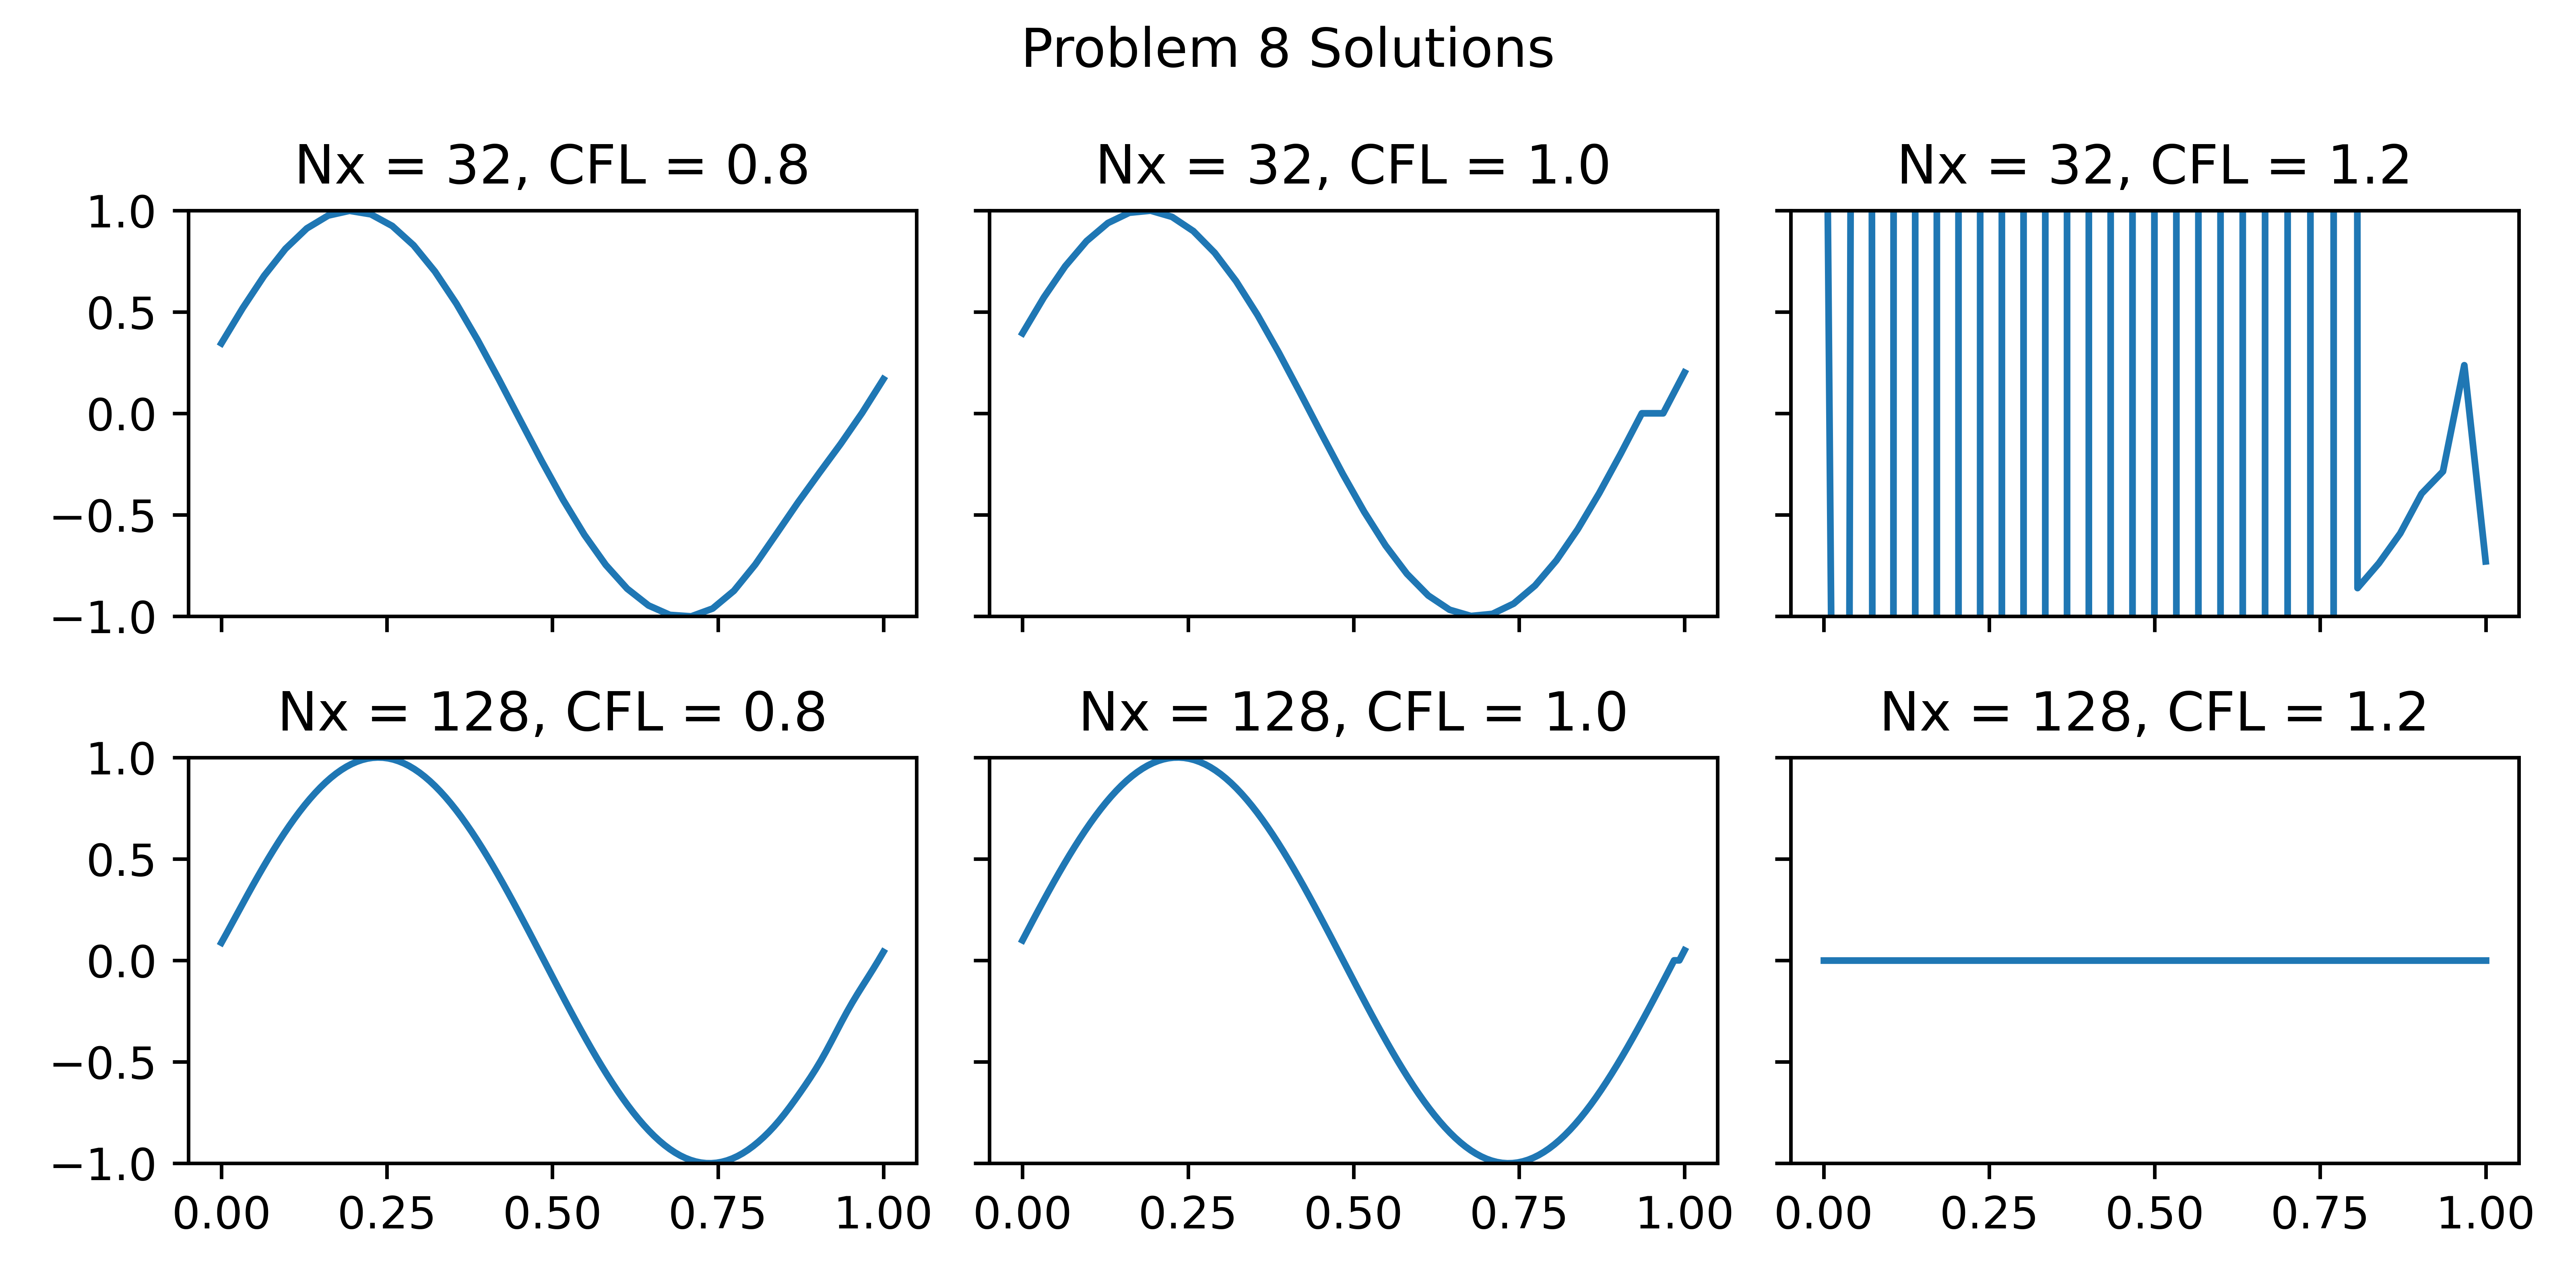
\includegraphics[width=\textwidth]{../code/prob8_tstop.png}
        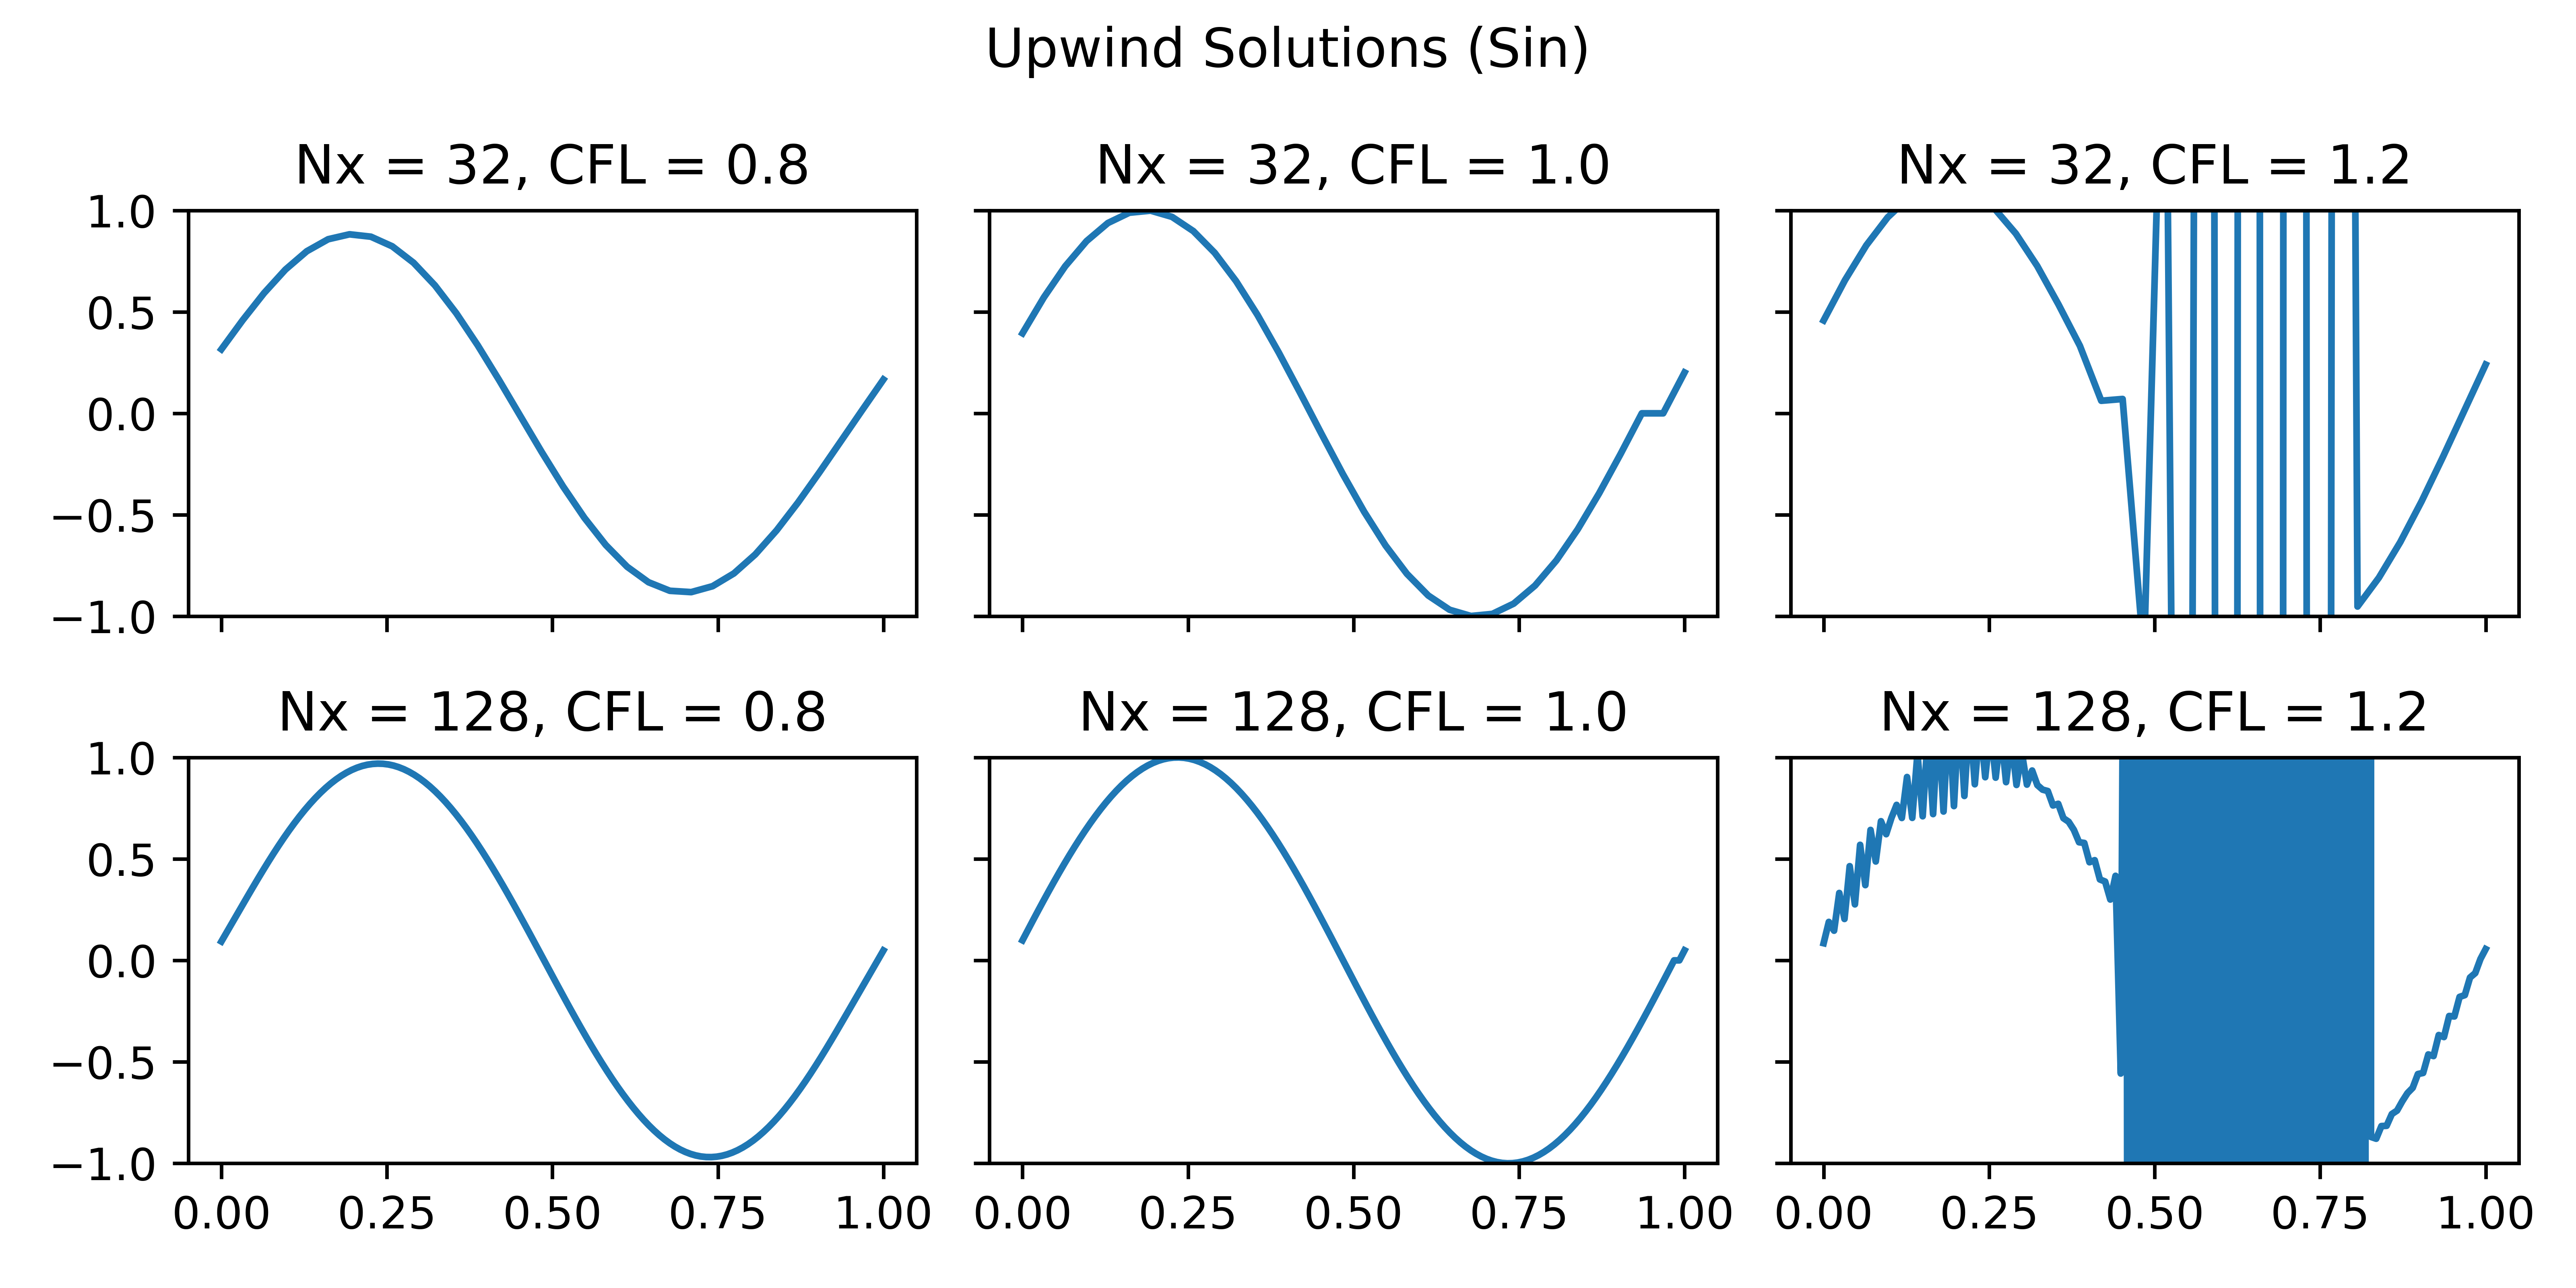
\includegraphics[width=\textwidth]{../code/upwind_sin_tstop.png}
    \emp
    \bmp{.49}
        \centering
        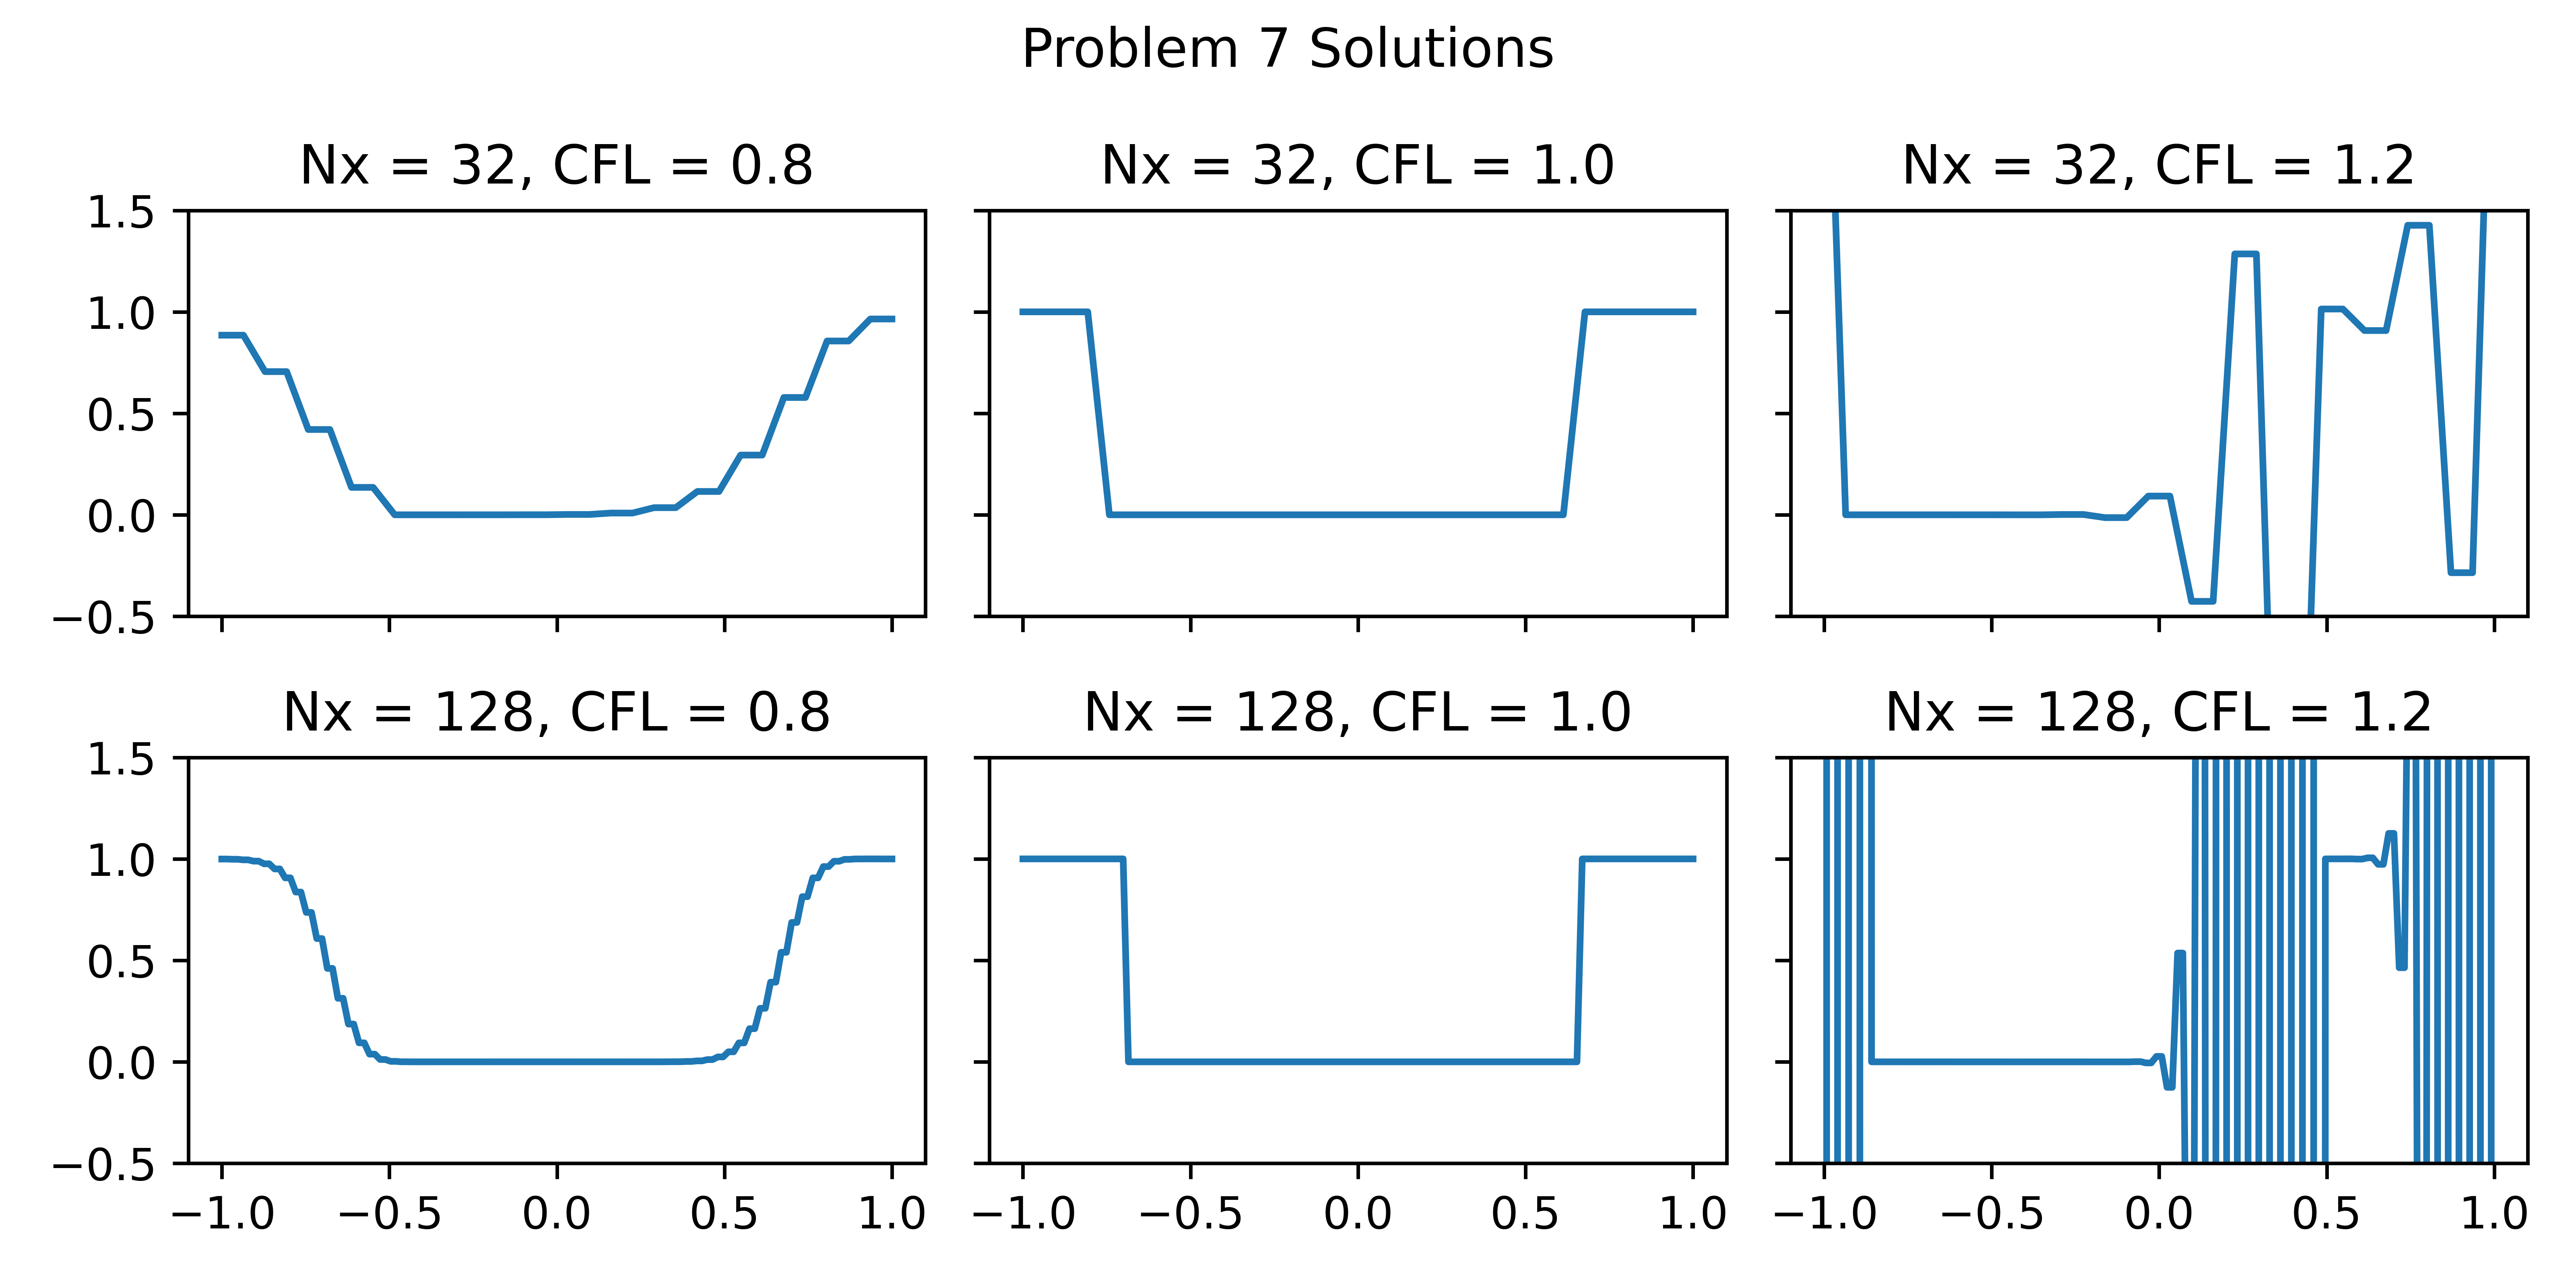
\includegraphics[width=\textwidth]{../code/prob7_tstop.png}
        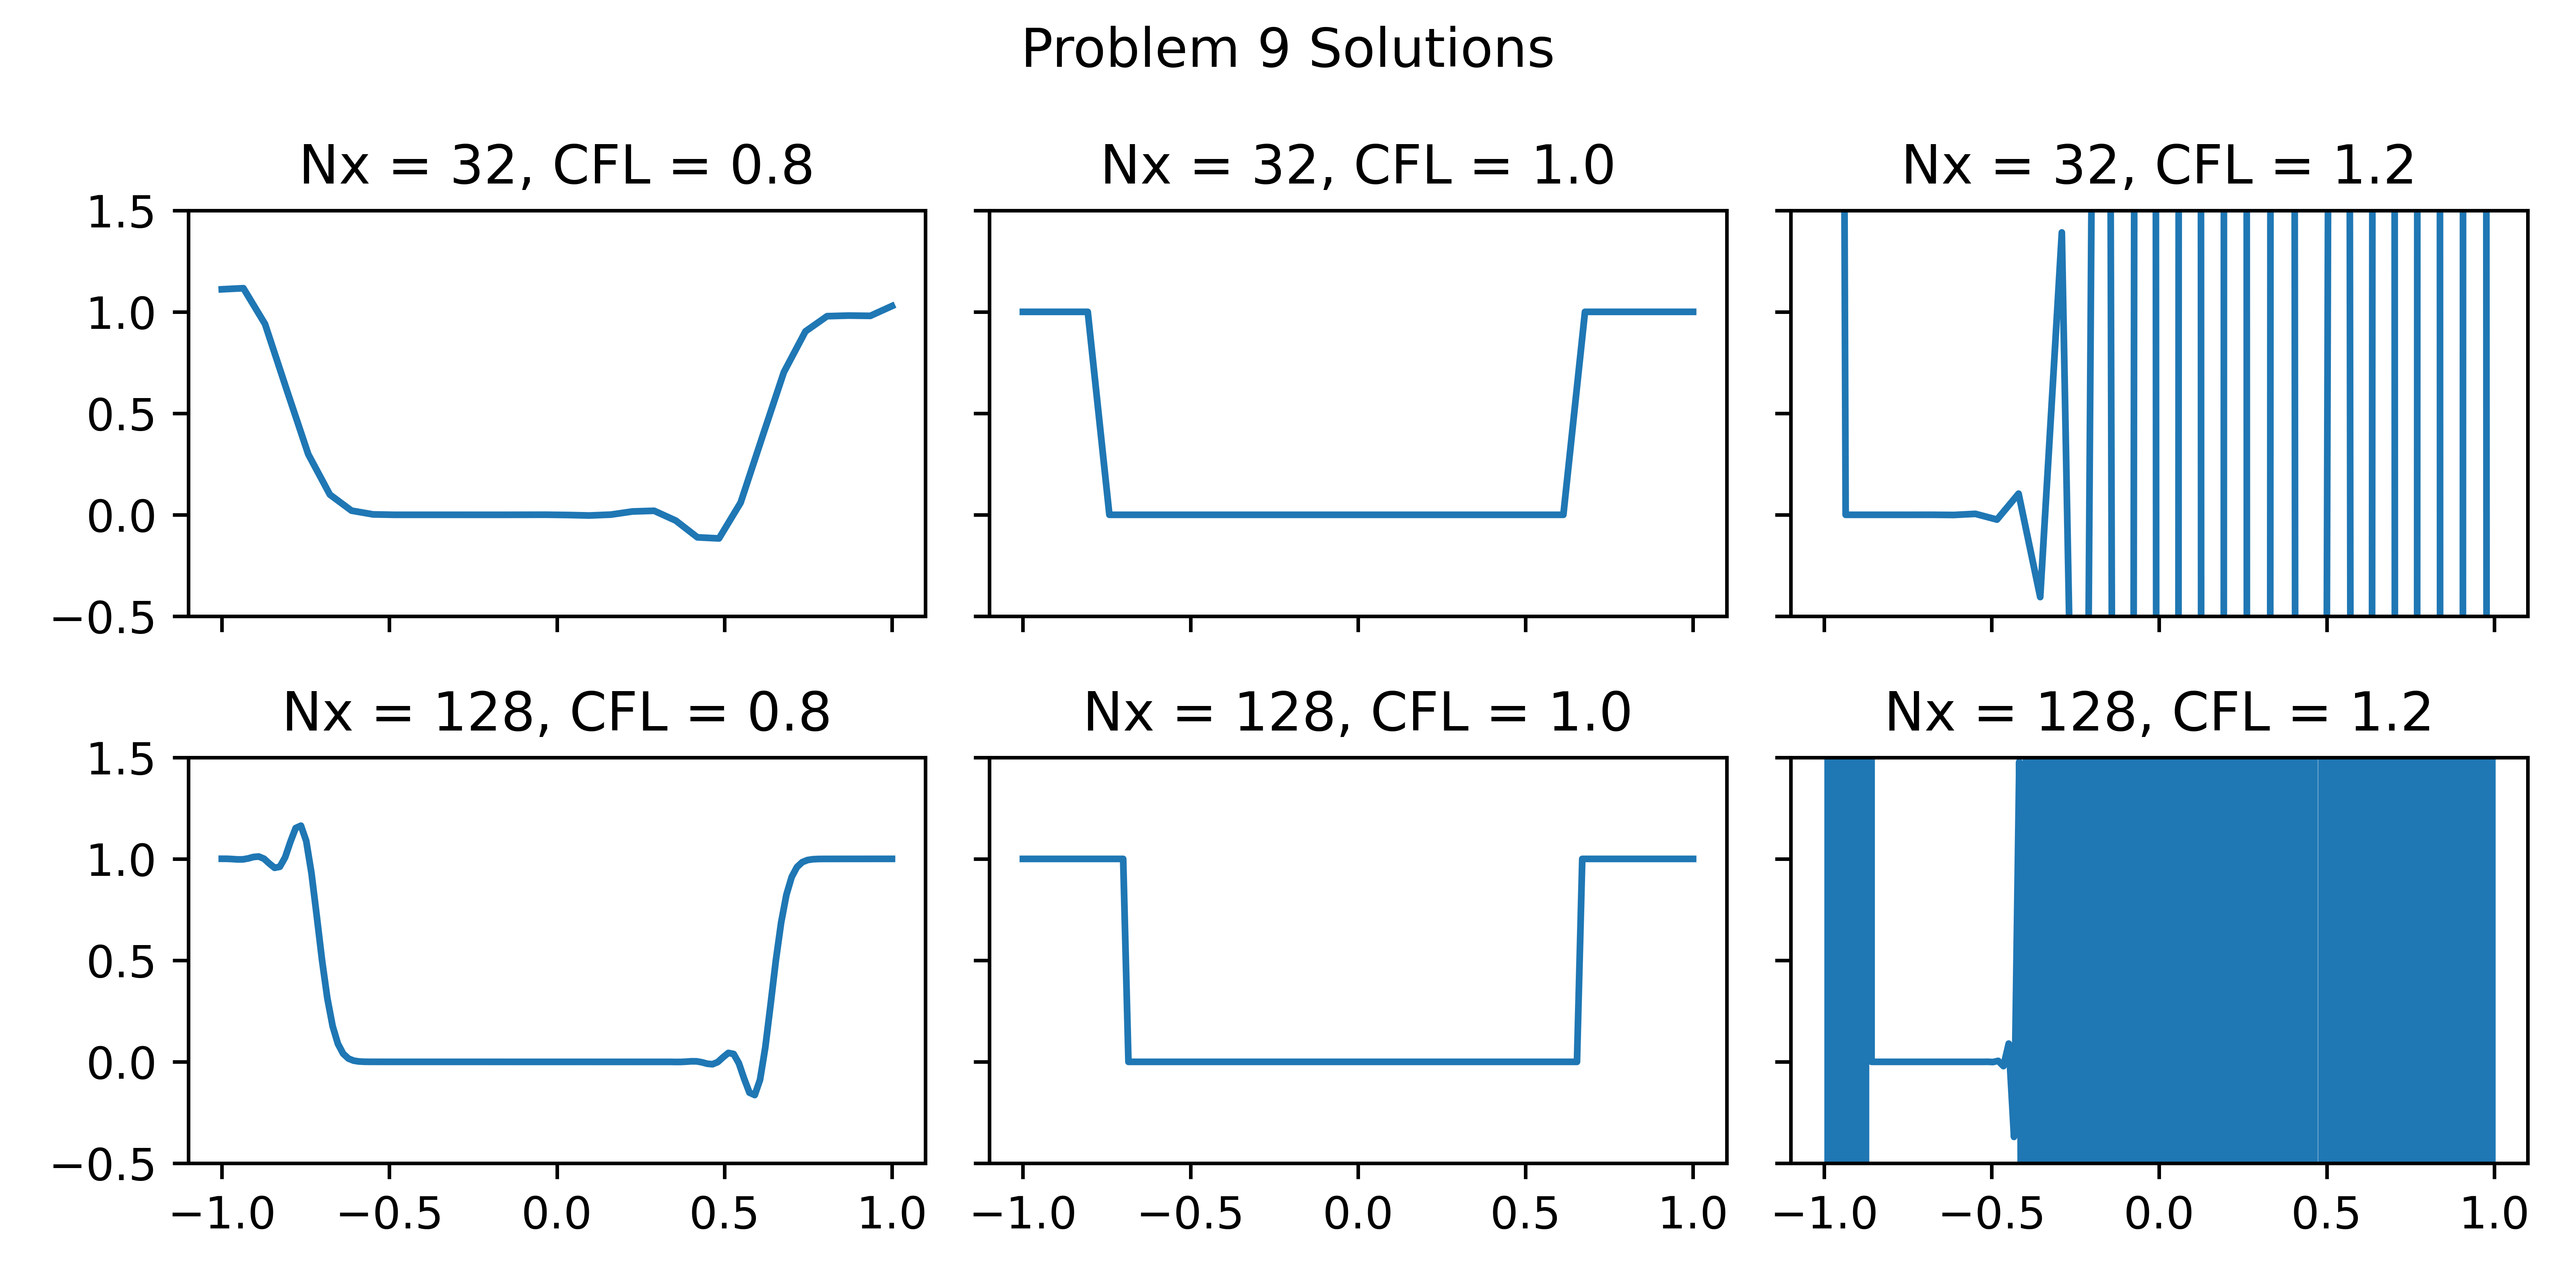
\includegraphics[width=\textwidth]{../code/prob9_tstop.png}
        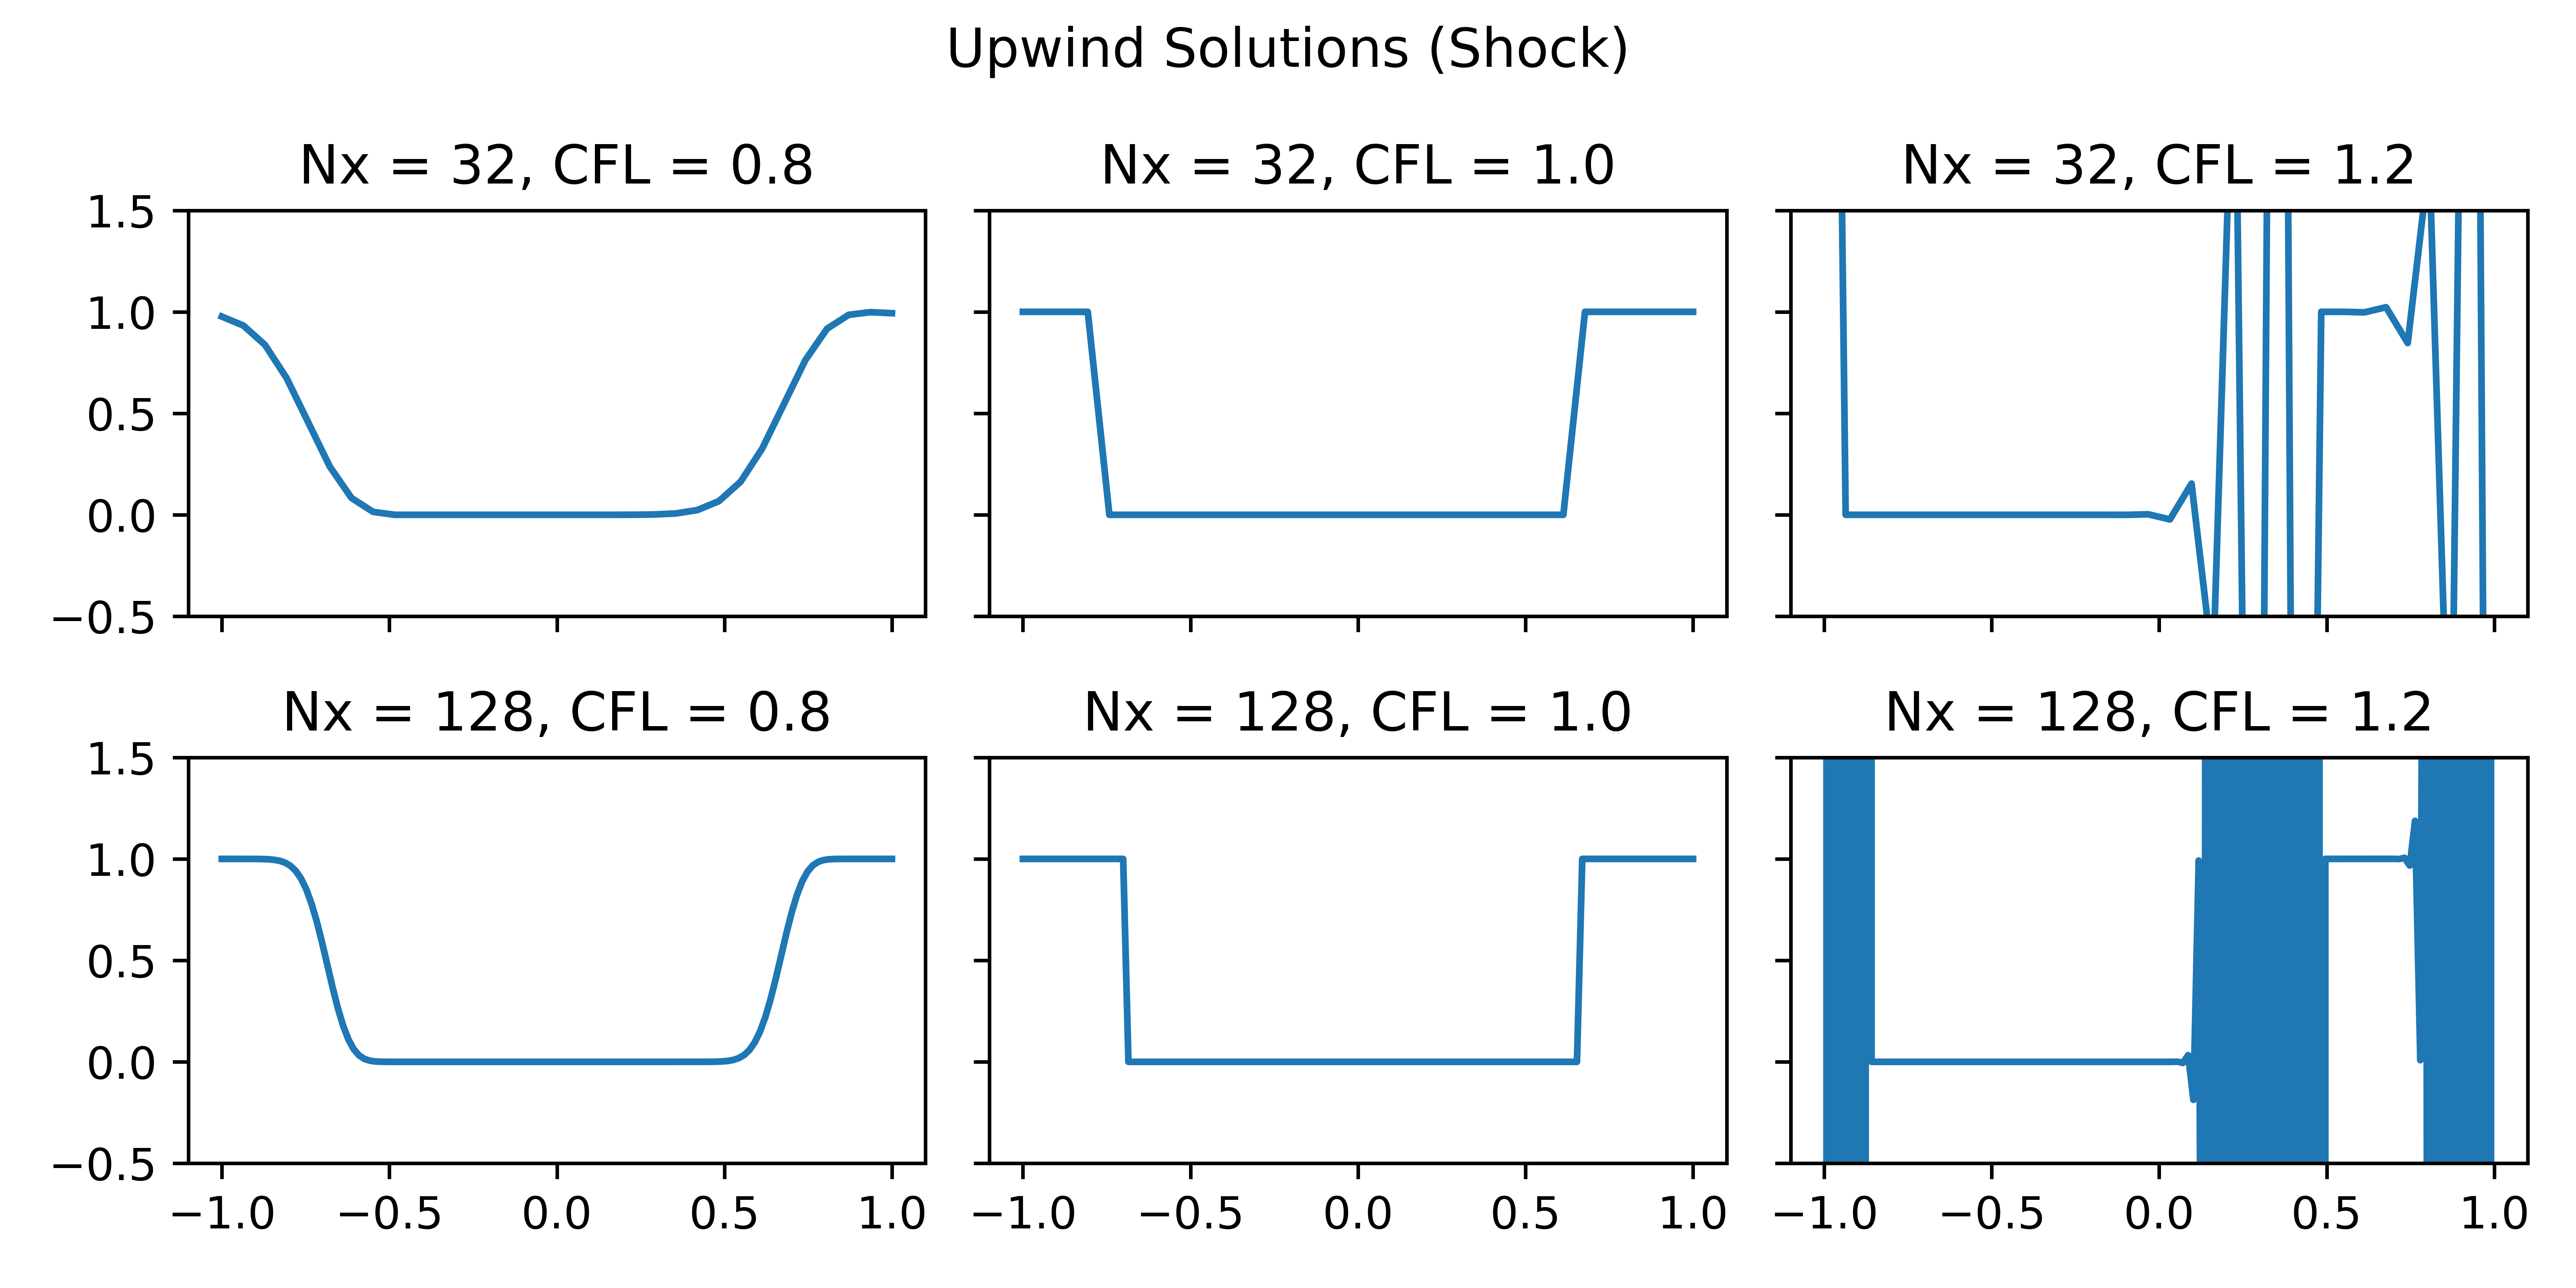
\includegraphics[width=\textwidth]{../code/upwind_shock_tstop.png}
    \emp
    \caption{Various initial conditions advected by Lax-Friedrichs Method (top),
    Lax-Wendroff Method (middle), and Upwind Method (bottom) for various grid sizes and
    CFL numbers. The left column shows the ``Sin Wave'' initial condition and
    the right column shows the ``Shock/Rarefraction Wave'' initial condition.}
    \label{fig:solutions}
\end{figure}

\section{Sinusoidal Adv. with LF}
My numerical implementation of the Lax-Friedrichs method for the sin wave initial
condition was done in Fortran and then
visualized using Python. The results can be seen in Figure \ref{fig:solutions}
alongside comparisions of the same solution using the Lax-Wendroff method and
the Upwind method. These are all plots of the solution at $t = t_{cycle}$ which
is computed by considering the advection speed compared to the natural
length scale of the system, i.e.
\begin{gather*}
    t_{cycle} = \frac{L_x}{c} = \frac{1}{1} = 1
\end{gather*}
Since the Lax-Friedrichs method is diffusive (as shown in an
earlier homework problem), we expect the amplitude of the sin wave to decrease
with time, which is indeed what we see for the lowest resolution result. As
expected, once the CFL number approaches and then increases past one, the
method is no longer stable. This is visualized by the oscillations seen in the
CFL = 1.2 plots. 

Compared to the upwind method, we see that the LF method appears to have slighly
worse errors for the same grid sizes. This is most apparent in the $CFL = 1.2$
cases where the oscillations away from the true solution have a much larger
length scale compared to the upwind solutions. Otherwise, the method seems to be
very similar to the upwind method. 


\section{Discontinuous IC with LF}

The same methodology and style of results for problem 6 can be seen in Figure
\ref{fig:solutions}. Here is LF method is used in the same way as before, only
with a different initial condition. Unlike before, where the upwind and LF
method appears to be very similar, we see that the LF is much worse at resolving
shocks and rarefraction waves. In the $Nx = 32$ and $CFL = 0.8$ we see very
jagged edges on the contour of the shock front and rarefraction fan. This
appears to be partially caused by the resolution of the system, but also speaks
to the inability of the method. The upwind method does not preserve the shock
front well either, but its solution is at least smooth. Both fail quite
spectacularly (as expected) at $CFL = 1.2$. 

\section{Sinusoidal Adv. with LW}

See Figure \ref{fig:solutions} for the results. Unlike the LF method, this
methods reaction to a large CFL number appears to to be quite erratic. The $Nx =
128$ and $CFL = 1.2$ appears to have diffused completely, while the $Nx = 32$
and $CFL = 1.2$ appears to have blown up completely. Besides this, the $CFL =
0.8, 1$ are very reasonable solutions and appear to be quite stable. 

\section{Discontinuous IC with LW}

See Figure \ref{fig:solutions} for the results. Perhaps the most interesting
aspect about the solutions to this method is that (because the method is not
diffusive), we notice rather than a degredation of the shock front /
rarefraction wave, we see oscillations (similar to Gibbs phenomenon) around the
discontinuity points. This is especially visible in the $Nx = 128$ and $CFL =
0.8$ plot. Again, the method appears to be highly sensitive to the $CFL$ number
(the $1.2$ plots particularly). If I've learned anything its that I should never
have a CFL number above $0.8$. 


\end{document}
